\documentclass[11pt]{article}

\usepackage[utf8]{inputenc}
\usepackage[italian]{babel}
\usepackage[T1]{fontenc}
\usepackage[a4paper,total={180mm, 267mm},left=10mm,top=10mm]{geometry}
\usepackage{fancyhdr, hyperref, graphicx}

\setlength{\parindent}{0pt}

\pagestyle{fancy}
\fancyhead{}
\fancyfoot{}
\fancyfoot[R]{\thepage}

\renewcommand{\headrulewidth}{0pt}
\renewcommand{\footrulewidth}{0pt}

\hypersetup{
    colorlinks=true,
    linktoc=all,
    linkcolor=black, 
}

\begin{document}
  \begin{titlepage}
    \vspace*{\fill}
    \centering

    \textbf{\Huge Regesta Dev Candidate Assessment}
    \vspace*{1.5cm}

    \textbf{\LARGE Alessandro Muscio}
    \vspace*{0.8cm}

    \begin{figure}[h]
      \centering
      
\includegraphics[]{../public/cropped-v2-icona-regesta-1-192x192.png}
    \end{figure}

    \Large User guide with all possible scenarios using the website

    \vspace*{\fill}
  \end{titlepage}

  \section*{User Guide}
  \subsection*{First page}
  When you open the website you will be faced with a standard \textit{form} in which you can fill the relative fields in order to search for your product.

  \begin{figure}[h]
    \centering
    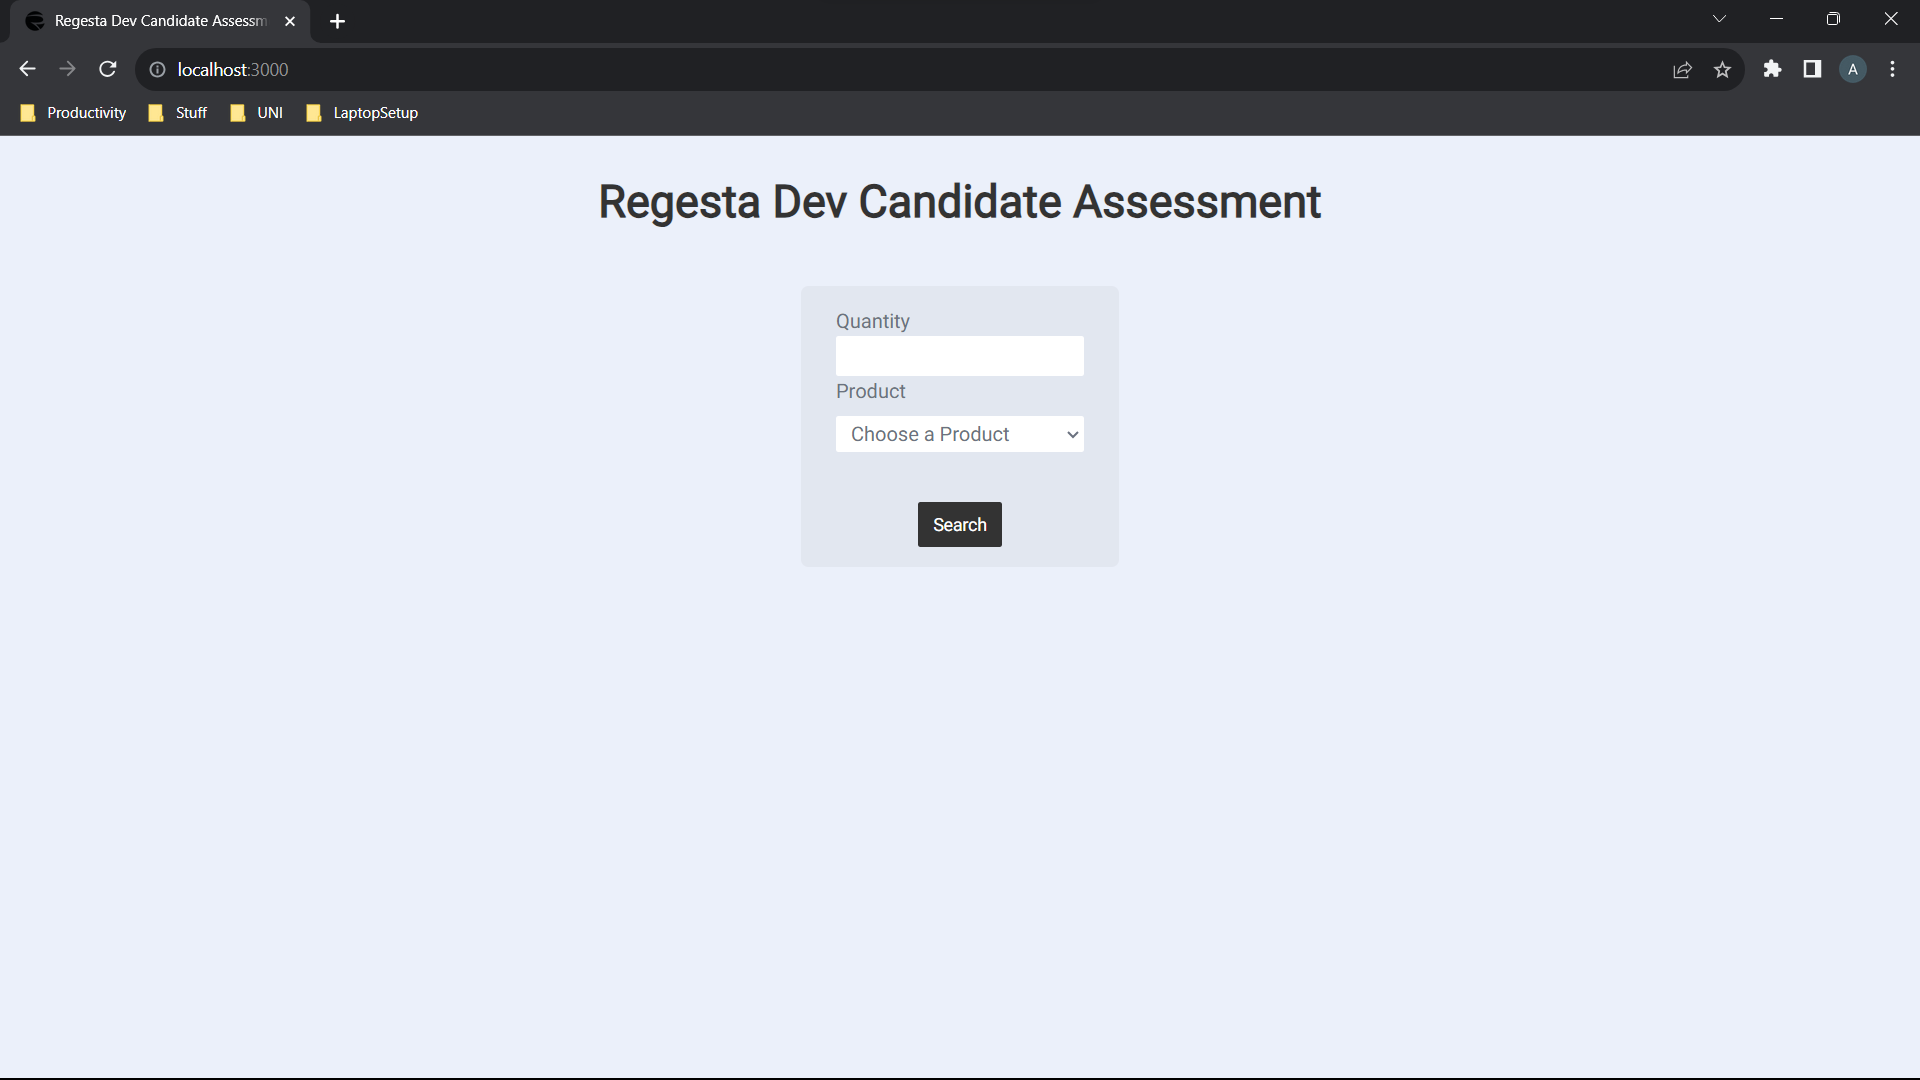
\includegraphics[scale=0.4433]{images/01.png}
  \end{figure}

  Here, as you can see from the above image, you can select the \underline{quantity} and the \underline{product name}.
  
  \subsection*{Selecting the Product}
  For the selection of the product you will have a \textbf{drop down menu} with all the products currently in the \textit{database}.

  \begin{figure}[h]
    \centering
    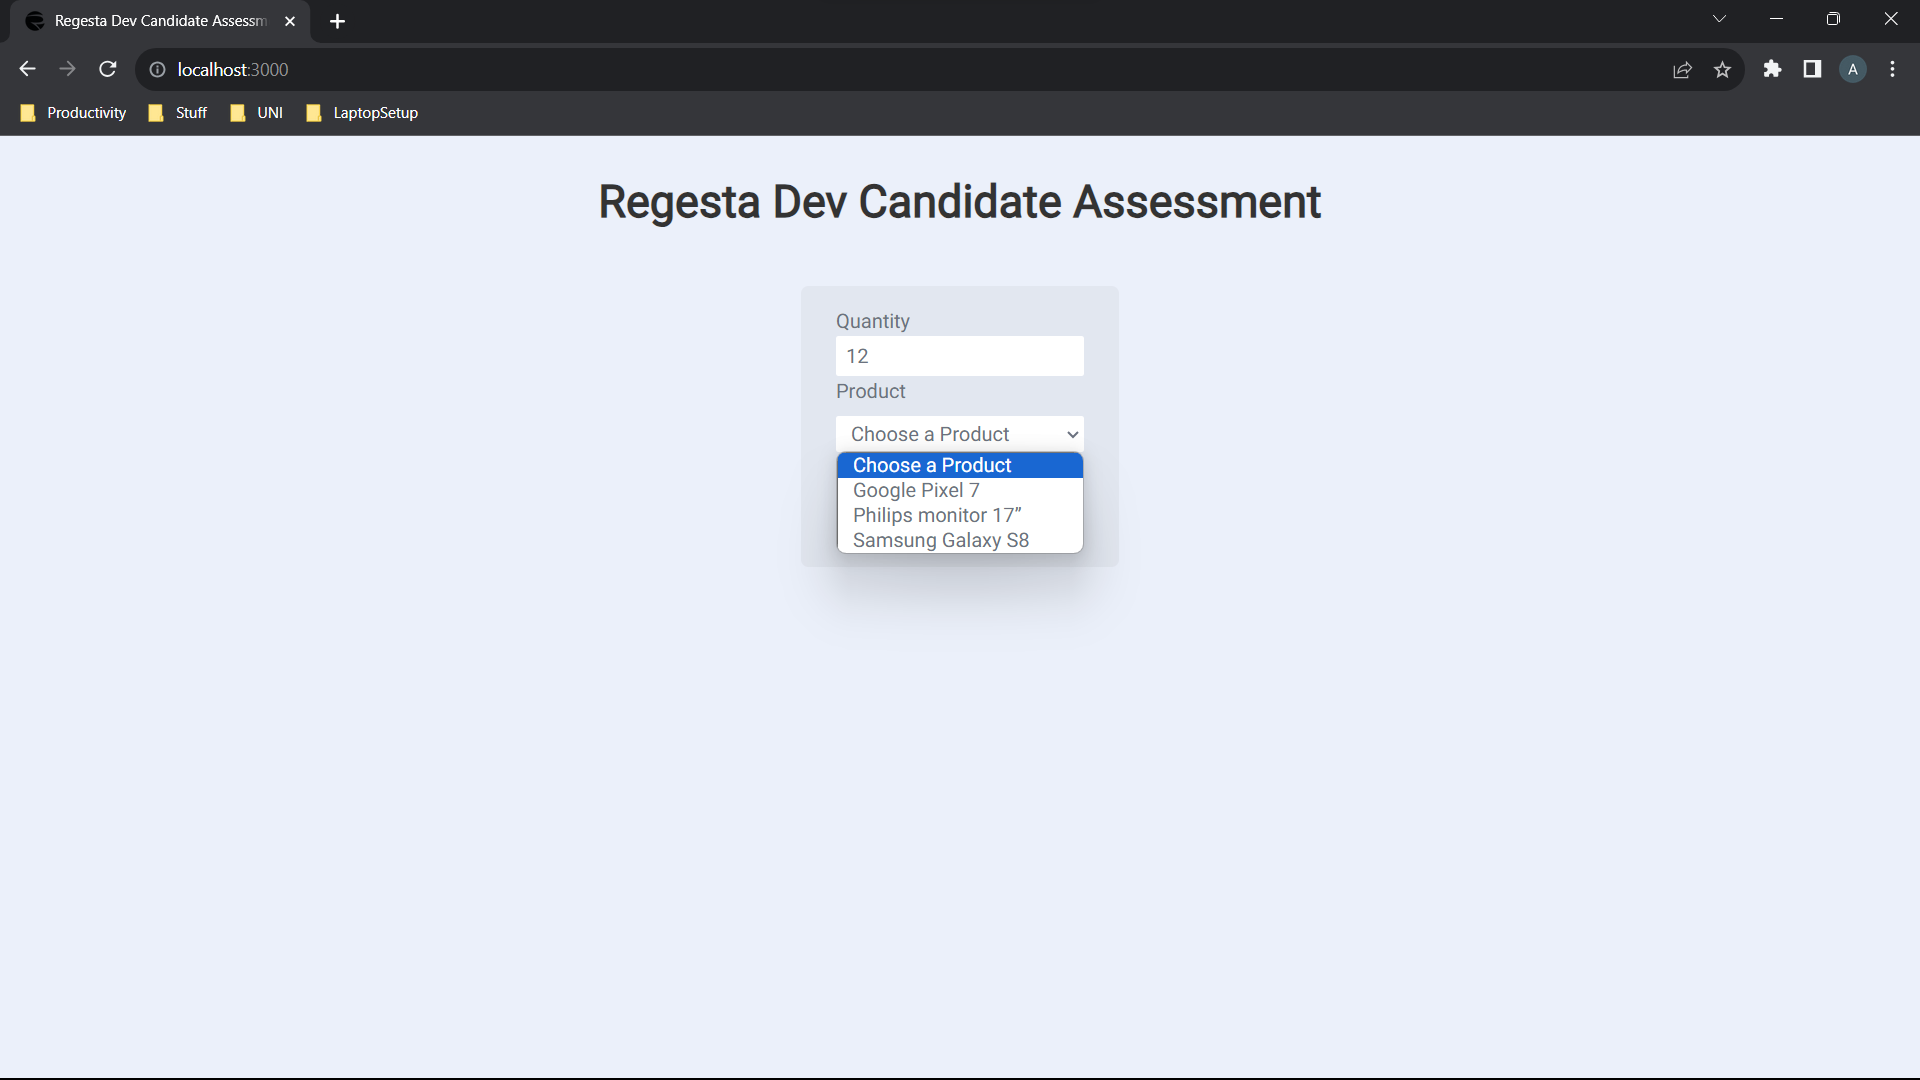
\includegraphics[height=9.0593cm]{images/02.png}
  \end{figure}

  After selecting your product, you can press the \textbf{search button} in order to start your search and go to the \textbf{Suppliers' Page}.

  \subsection*{Suppliers' Page}
  In the \textbf{suppliers' page} you can have two scenarios:
  \begin{itemize}
    \item \textbf{Error}: your search went wrong
    \item \textbf{Success}: everything went fine
  \end{itemize}

  \subsubsection*{Error Scenario}
  This is pretty straightforward, it's a generic error page that can happen due to different circumstances, ranging from a \textit{server error} to a request that was \textit{parsed} in the wrong way.

  \begin{figure}[h]
    \centering
    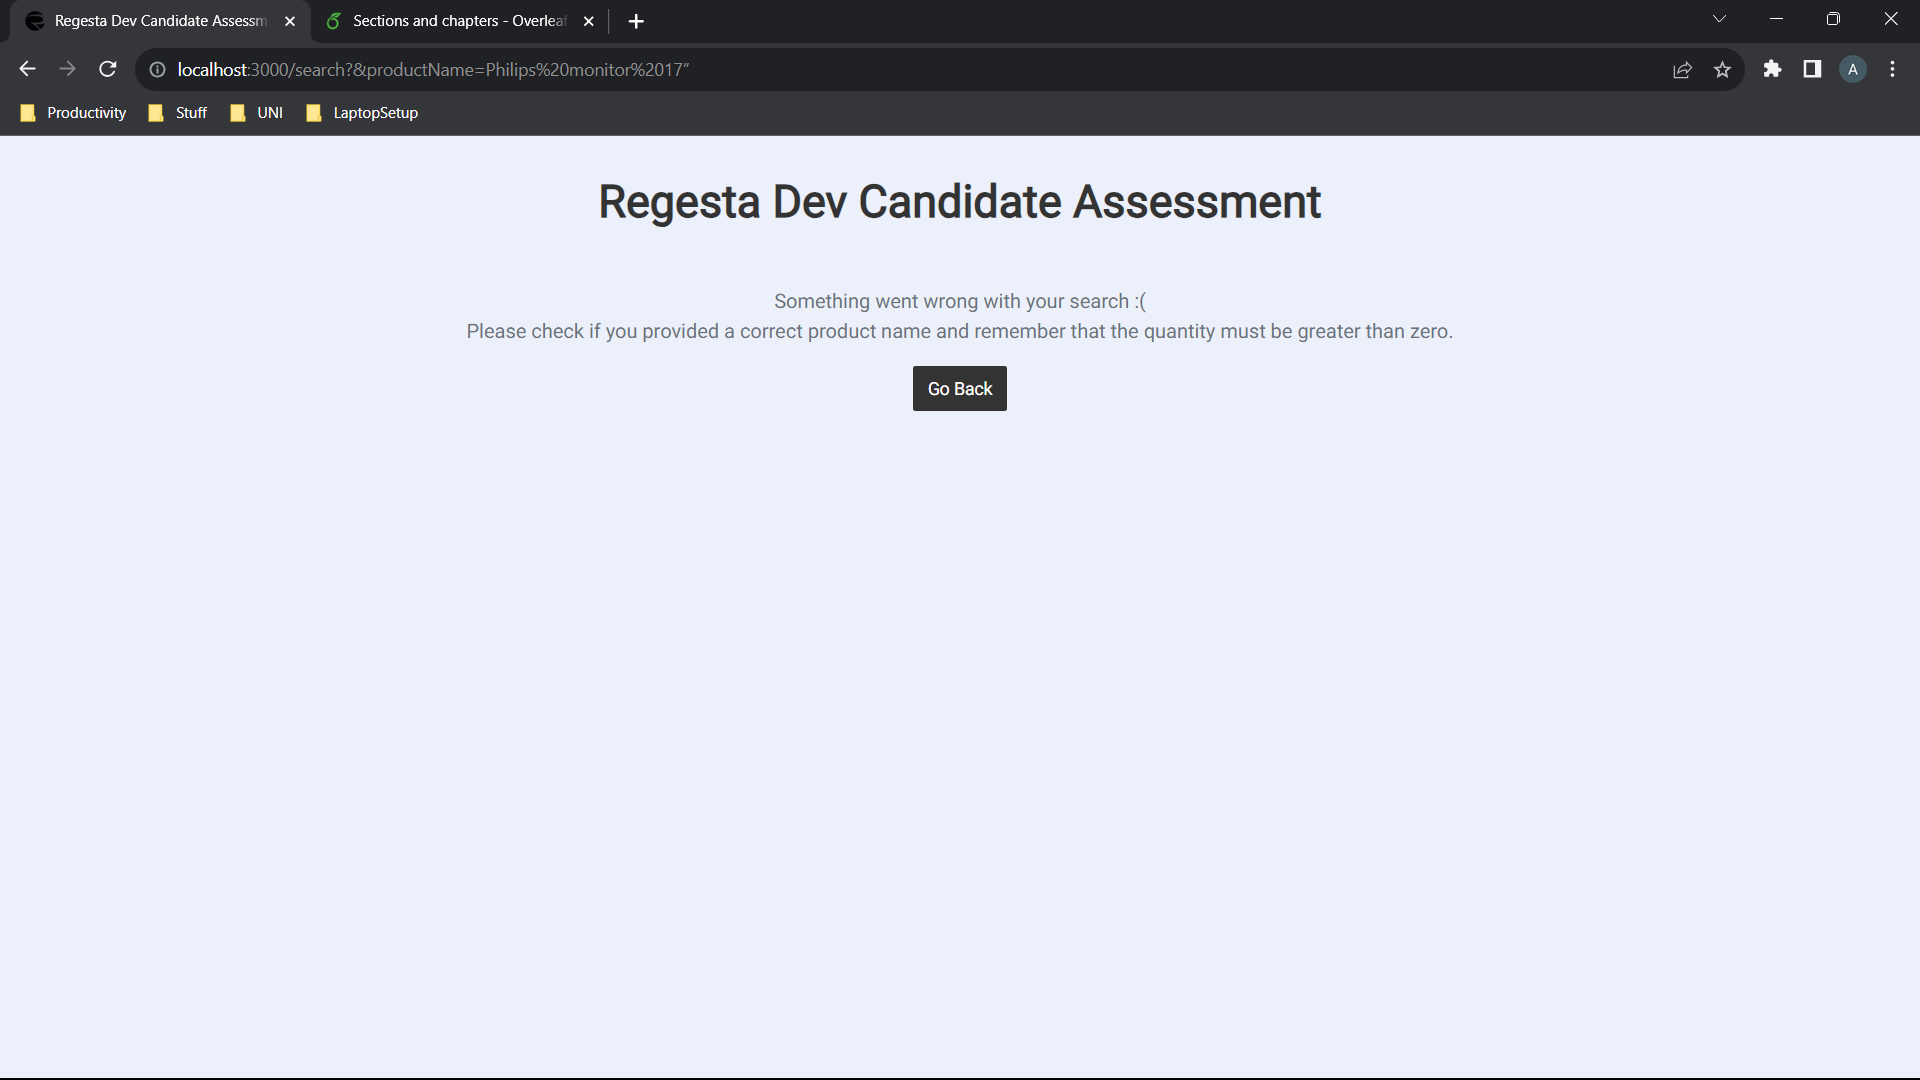
\includegraphics[scale=0.4433]{images/03.png}
  \end{figure}

  \subsubsection*{Success Scenario}
  In here everything went smoothly and the request was received by the server. Here you can also have two different responses: 
  \begin{itemize}
    \item \textbf{Not Found}: the product wasn't found
    \item \textbf{Found}: the product was found
  \end{itemize}
  \newpage

  \paragraph*{Not Found}
  If you got here it means that the product you searched for wasn't available in the quantity you specified.

  \begin{figure}[h]
    \centering
    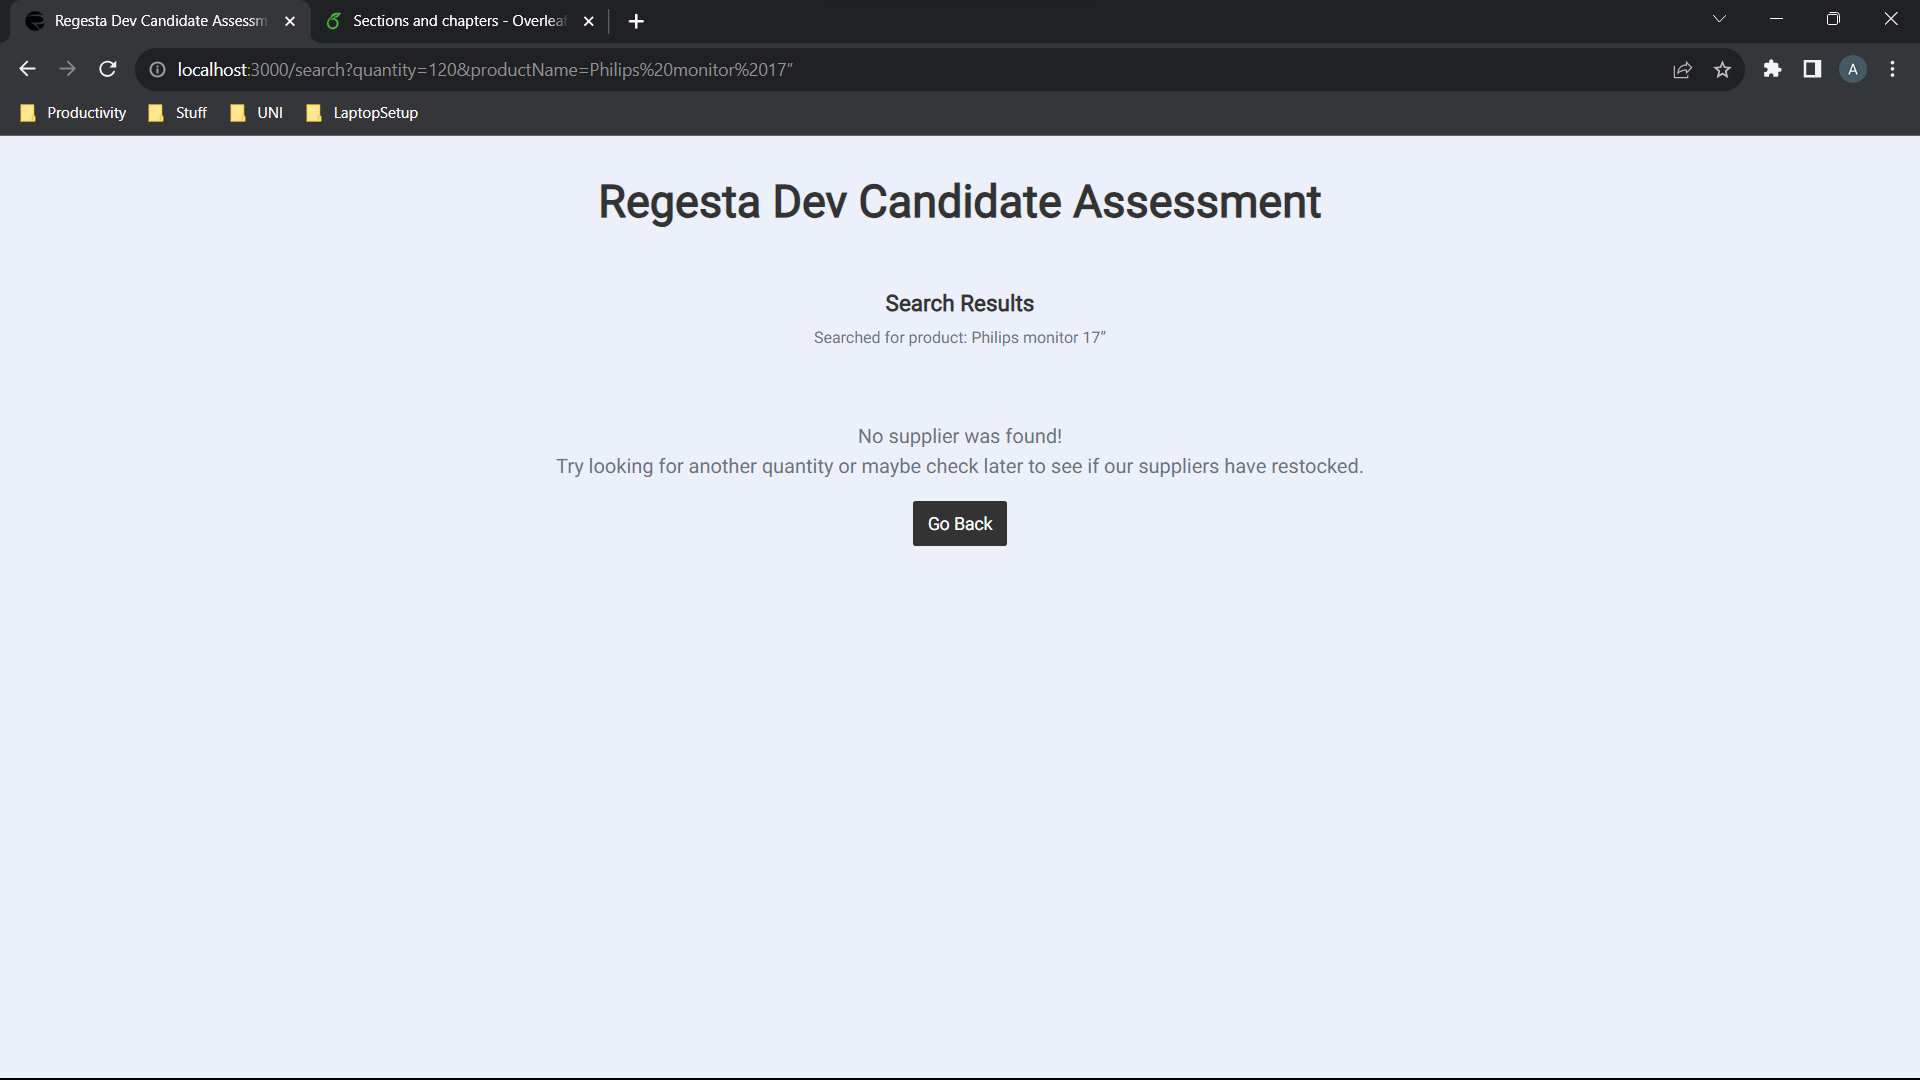
\includegraphics[scale=0.4433]{images/04.png}
  \end{figure}

  \paragraph*{Found}
  This is the desired scenario and, hopefully, the one you will always see. In here you'll see a list of suppliers who do sell the product you searched for in that quantity, all sorted from the cheapest to the most expensive one, with also the estimated days needed to fulfil the order.

  The first, and cheapest one, will also be highlighted and marked as the cheapest like shown in the image below.

  \begin{figure}[h]
    \centering
    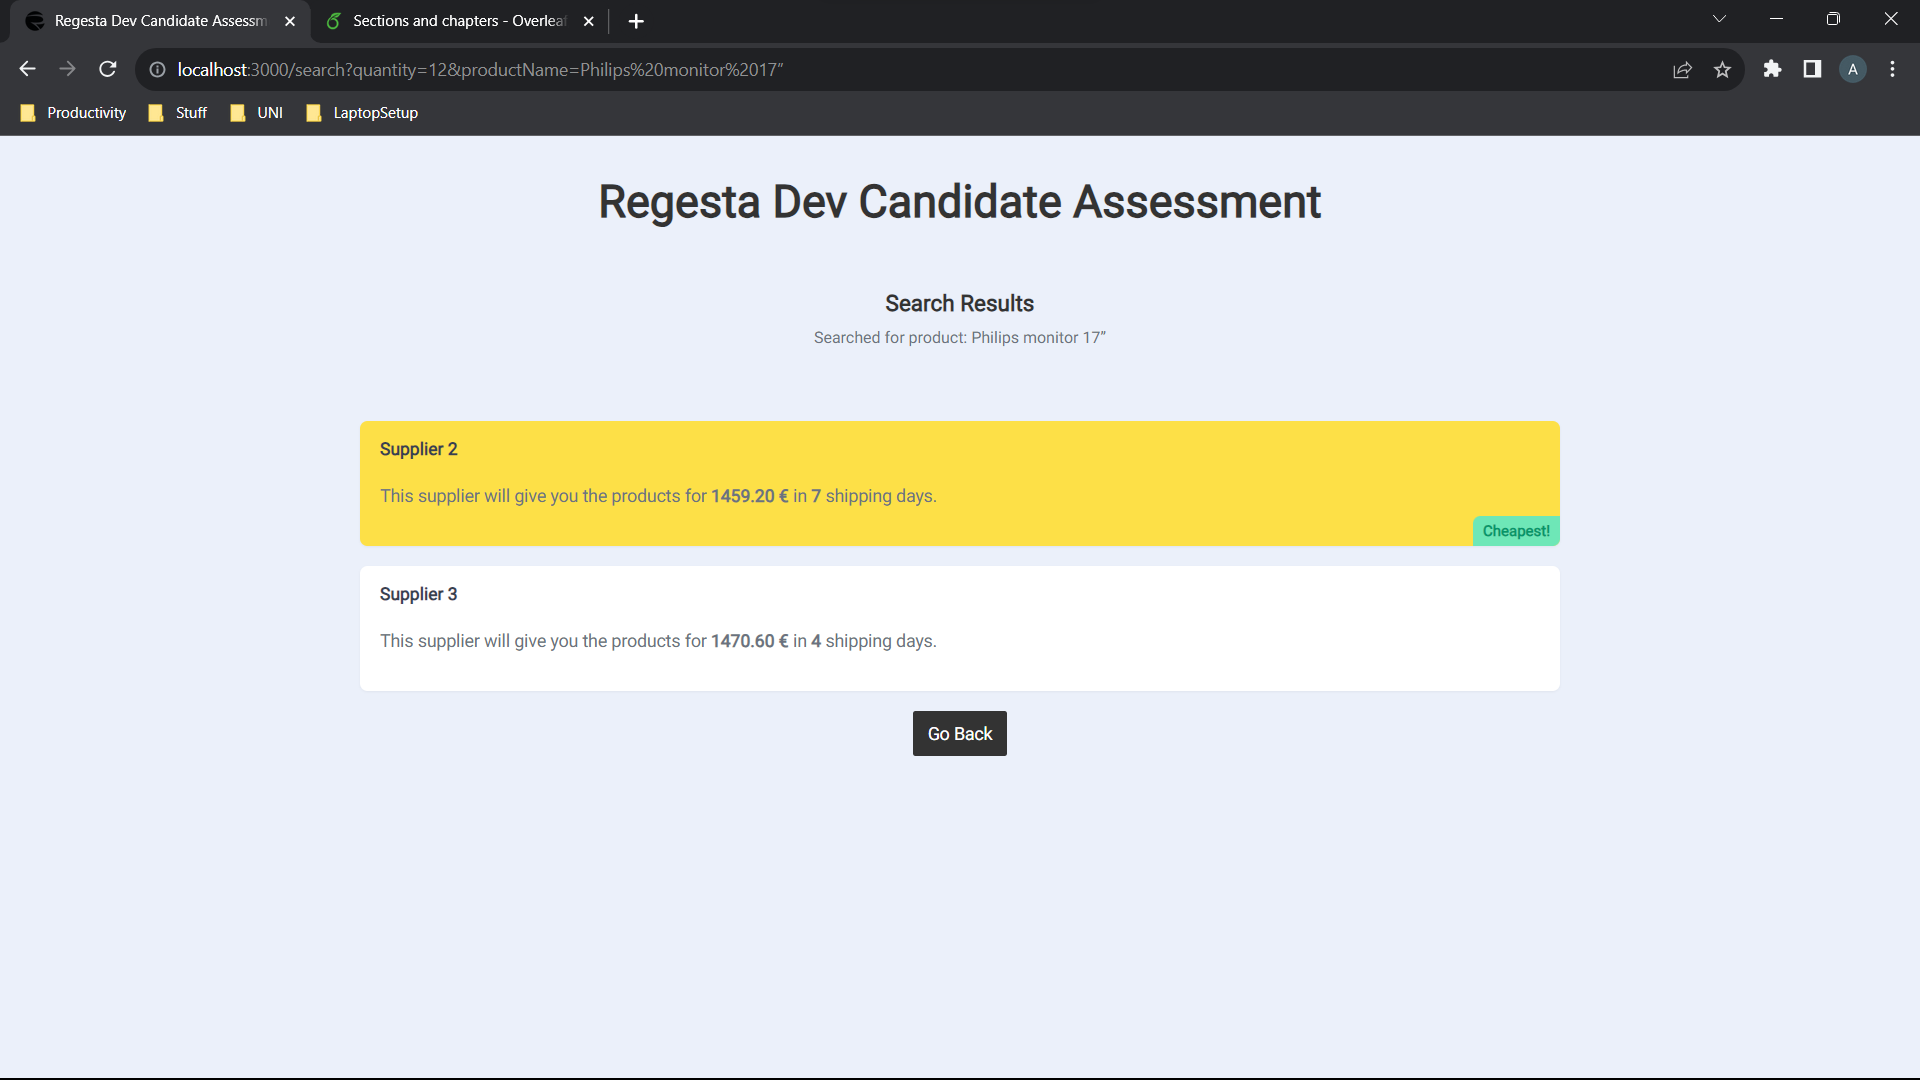
\includegraphics[height=9.9601cm]{images/05.png}
  \end{figure}
\end{document}
